\section{Arquitetura Intel x86}

\begin{frame}[fragile]{Registradores x86}

    \begin{itemize}
        \item Um dos principais motivos do sucesso da linha de processadores x86 da Intel foi
            o fato de que eles foram desenvolvidos para serem sempre compatíveis com os seus
            antecessores

        \item Deste modo, eram minimizadas as alterações em hardware e software necessárias para
            que um software desenvolvido para um processador fossem portado e funcionasse em
            futuras iterações desta arquitetura

        \item Os concorrentes que optam por começar do zero em determinadas iterações (como a 
            Motorola e a IBM com os chips PowerPC e a DEC com os processadores Alpha) acabaram
            não obtendo o mesmo sucesso a longo prazo

        \item O estudo dos registradores x86, neste sentido, ganha um aspecto histórico
    \end{itemize}

\end{frame}

\begin{frame}[fragile]{Registradores 8080}

    \begin{itemize}
        \item Os processadores 8080 foram os primeiros a serem produzidos em massa

        \item O primeiro computador pessoal (Altair, em 1975) utilizava um processador 8080

        \item Ele possuía 6 registradores de 8-\textit{bits}: $A, B, C, D, H, L$ 

        \item Os endereços de memória e a transferência de dados também eram de 8-\textit{bits}

        \item O registrador $L$ (\textit{low}) armazenava endereços de memória, e a memória era 
            composta de 256-\textit{bytes}, identificados pelos números de 0 a 255

        \item Este registrador poderia ser combinado com o registrador $H$ (\textit{high}) para
            compôr um endereço de 16-\textit{bits}

        \item Quando este par era referenciado por uma instrução, ela utiliza a letra $X$ 
            (\textit{extended}) para sinalizar este uso
    \end{itemize}

\end{frame}

\begin{frame}[fragile]{Visualização do 8080}

    \begin{figure}[ht]
        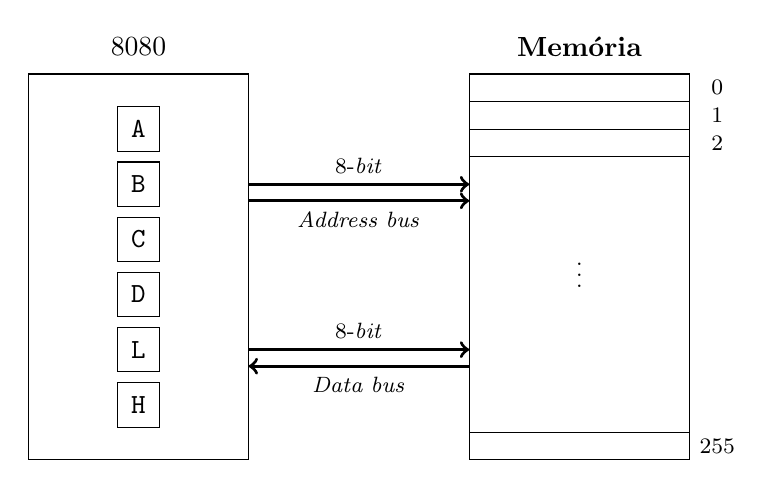
\begin{tikzpicture}[scale=0.7]
            \coordinate (A1) at (0, 8);
            \coordinate (B1) at (4, 8);
            \coordinate (C1) at (4, 1);
            \coordinate (D1) at (0, 1);

            \draw (A1) -- (B1) -- (C1) -- (D1) -- (A1);
            \node at (2, 8.5) { $8080$ };

            \node[draw,inner sep=5pt] at (2, 7) { \tt A };
            \node[draw,inner sep=5pt] at (2, 6) { \tt B };
            \node[draw,inner sep=5pt] at (2, 5) { \tt C };
            \node[draw,inner sep=5pt] at (2, 4) { \tt D };
            \node[draw,inner sep=5pt] at (2, 3) { \tt L };
            \node[draw,inner sep=5pt] at (2, 2) { \tt H };

            \coordinate (A2) at (8, 8);
            \coordinate (B2) at (12, 8);
            \coordinate (C2) at (12, 1);
            \coordinate (D2) at (8, 1);

            \coordinate (A3) at (8, 8);
            \coordinate (B3) at (12, 8);
            \coordinate (C3) at (12, 7.5);
            \coordinate (D3) at (8, 7.5);

            \coordinate (A4) at (8, 7.5);
            \coordinate (B4) at (12, 7.5);
            \coordinate (C4) at (12, 7);
            \coordinate (D4) at (8, 7);

            \coordinate (A5) at (8, 7);
            \coordinate (B5) at (12, 7);
            \coordinate (C5) at (12, 6.5);
            \coordinate (D5) at (8, 6.5);

            \coordinate (A6) at (8, 1.5);
            \coordinate (B6) at (12, 1.5);
            \coordinate (C6) at (12, 1);
            \coordinate (D6) at (8, 1);

            \draw (A2) -- (B2) -- (C2) -- (D2) -- (A2);
            \draw (A3) -- (B3) -- (C3) -- (D3) -- (A3);
            \draw (A4) -- (B4) -- (C4) -- (D4) -- (A4);
            \draw (A5) -- (B5) -- (C5) -- (D5) -- (A5);
            \draw (A6) -- (B6) -- (C6) -- (D6) -- (A6);

            \node at (10, 8.5) { \bf Memória };
            \node at (12.5, 7.75) { \footnotesize $0$ };
            \node at (12.5, 7.25) { \footnotesize $1$ };
            \node at (12.5, 6.75) { \footnotesize $2$ };
            \node at (12.5, 1.25) { \footnotesize $255$ };
            \node at (10, 4.5) { \footnotesize $\vdots$ };
        
            \draw[->,very thick] (4, 6) -- node[anchor=south] { \footnotesize 8-\textit{bit} } (8, 6);
            \draw[->,very thick] (4, 5.7) -- node[anchor=north] { \footnotesize \textit{Address bus} } (8, 5.7); 
            \draw[->,very thick] (4, 3) -- node[anchor=south] { \footnotesize 8-\textit{bit} } (8, 3);
            \draw[<-,very thick] (4, 2.7) -- node[anchor=north] { \footnotesize \textit{Data bus} } (8, 2.7);
        \end{tikzpicture}
        \caption{Visualização de um computador com processador 8080.\footnote{Fonte: \textbf{NEVELN}, Bob. \textit{Linux Assembly Language Programming}, Open Source Technology Series, Prentice-Hall, 2000 (com adaptações).}}
    \end{figure}

\end{frame}

\begin{frame}[fragile]{Registradores 8086}

    \begin{itemize}
        \item Quando o processador de 16-\textit{bits} 8086 foi desenvolvido, a letra $X$ foi 
            usada para designar os novos registradores de 16-\textit{bits}: $AX, BX, CX$ e $DX$

        \item Estes novos registradores são pares de registradores de 8-\textit{bits}: $AL, AH,
            BL, BH, CL, CH, DL$ e $DH$

        \item Os demais registradores de 16-\textit{bits}, a saber: $SP, BP, SI$ e $DI$, não são
            pares, e não trazem a letra $X$ em sua nomenclatura

        \item A transferência de dados é feita em 16-\textit{bits}

        \item Contudo, o endereçamento de memória é feito em 20-\textit{bits}, porém sem uma
            forma eficiente de usar todos estes \textit{bits} de uma só vez
    \end{itemize}

\end{frame}

\begin{frame}[fragile]{Visualização parcial do 8086}

    \begin{figure}[ht]
        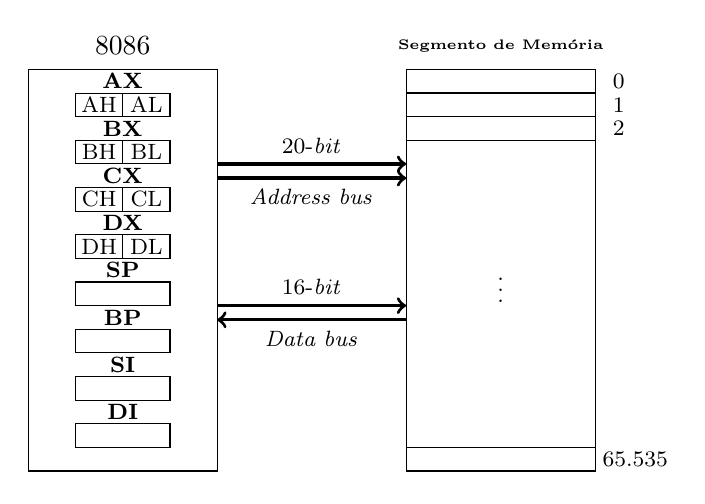
\begin{tikzpicture}[scale=0.6]
            \coordinate (A1) at (0, 8);
            \coordinate (B1) at (4, 8);
            \coordinate (C1) at (4, -0.5);
            \coordinate (D1) at (0, -0.5);

            \draw (A1) -- (B1) -- (C1) -- (D1) -- (A1);
            \node at (2, 8.5) { $8086$ };

            \draw (1, 7) rectangle (2, 7.5);
            \draw (2, 7) rectangle (3, 7.5);
            \node at (1.5, 7.25) { \footnotesize AH };
            \node at (2.5, 7.25) { \footnotesize AL };
            \node at (2, 7.75) { \footnotesize \bf AX };

            \draw (1, 6) rectangle (2, 6.5);
            \draw (2, 6) rectangle (3, 6.5);
            \node at (1.5, 6.25) { \footnotesize BH };
            \node at (2.5, 6.25) { \footnotesize BL };
            \node at (2, 6.75) { \footnotesize \bf BX };

            \draw (1, 5) rectangle (2, 5.5);
            \draw (2, 5) rectangle (3, 5.5);
            \node at (1.5, 5.25) { \footnotesize CH };
            \node at (2.5, 5.25) { \footnotesize CL };
            \node at (2, 5.75) { \footnotesize \bf CX };

            \draw (1, 4) rectangle (2, 4.5);
            \draw (2, 4) rectangle (3, 4.5);
            \node at (1.5, 4.25) { \footnotesize DH };
            \node at (2.5, 4.25) { \footnotesize DL };
            \node at (2, 4.75) { \footnotesize \bf DX };

            \draw (1, 3) rectangle (3, 3.5);
            \node at (2, 3.75) { \footnotesize \bf SP };

            \draw (1, 2) rectangle (3, 2.5);
            \node at (2, 2.75) { \footnotesize \bf BP };

            \draw (1, 1) rectangle (3, 1.5);
            \node at (2, 1.75) { \footnotesize \bf SI };

            \draw (1, 0) rectangle (3, 0.5);
            \node at (2, 0.75) { \footnotesize \bf DI };

            \coordinate (A2) at (8, 8);
            \coordinate (B2) at (12, 8);
            \coordinate (C2) at (12, -0.5);
            \coordinate (D2) at (8, -0.5);

            \coordinate (A3) at (8, 8);
            \coordinate (B3) at (12, 8);
            \coordinate (C3) at (12, 7.5);
            \coordinate (D3) at (8, 7.5);

            \coordinate (A4) at (8, 7.5);
            \coordinate (B4) at (12, 7.5);
            \coordinate (C4) at (12, 7);
            \coordinate (D4) at (8, 7);

            \coordinate (A5) at (8, 7);
            \coordinate (B5) at (12, 7);
            \coordinate (C5) at (12, 6.5);
            \coordinate (D5) at (8, 6.5);

            \coordinate (A6) at (8, 0);
            \coordinate (B6) at (12, 0);
            \coordinate (C6) at (12, -0.5);
            \coordinate (D6) at (8, -0.5);

            \draw (A2) -- (B2) -- (C2) -- (D2) -- (A2);
            \draw (A3) -- (B3) -- (C3) -- (D3) -- (A3);
            \draw (A4) -- (B4) -- (C4) -- (D4) -- (A4);
            \draw (A5) -- (B5) -- (C5) -- (D5) -- (A5);
            \draw (A6) -- (B6) -- (C6) -- (D6) -- (A6);

            \node at (10, 8.5) { \tiny \bf Segmento de Memória };
            \node at (12.5, 7.75) { \footnotesize $0$ };
            \node at (12.5, 7.25) { \footnotesize $1$ };
            \node at (12.5, 6.75) { \footnotesize $2$ };
            \node at (12.85, -0.25) { \footnotesize $65.535$ };
            \node at (10, 3.5) { \footnotesize $\vdots$ };
        
            \draw[->,very thick] (4, 6) -- node[anchor=south] { \footnotesize 20-\textit{bit} } (8, 6);
            \draw[->,very thick] (4, 5.7) -- node[anchor=north] { \footnotesize \textit{Address bus} } (8, 5.7); 
            \draw[->,very thick] (4, 3) -- node[anchor=south] { \footnotesize 16-\textit{bit} } (8, 3);
            \draw[<-,very thick] (4, 2.7) -- node[anchor=north] { \footnotesize \textit{Data bus} } (8, 2.7);
        \end{tikzpicture}
        \caption{Visualização parcial de um computador com processador 8086.\footnote{Fonte: \textbf{NEVELN}, Bob. \textit{Linux Assembly Language Programming}, Open Source Technology Series, Prentice-Hall, 2000 (com adaptações).}}
    \end{figure}

\end{frame}

\begin{frame}[fragile]{Registradores 80386}

    \begin{itemize}
        \item A arquitetura dos processadores 8086 foi aperfeiçoada nos novos processadores 80386

        \item Os oito registradores que iniciam com a letra $E$ (\textit{extension}) são extensões
            dos registradores do 8086

        \item Cada registrador tem 32-\textit{bits}, e seus 16-\textit{bits} menos significativos
            correspondem ao registradores do 8086

        \item A transferência de dados e o endereçamento de memória são feitos em 32-\textit{bits}

        \item Os processadores 80486 e Pentium também são computadores de 32-\textit{bits}
    \end{itemize}

\end{frame}

\begin{frame}[fragile]{Visualização parcial do 80386}

    \begin{figure}[ht]
        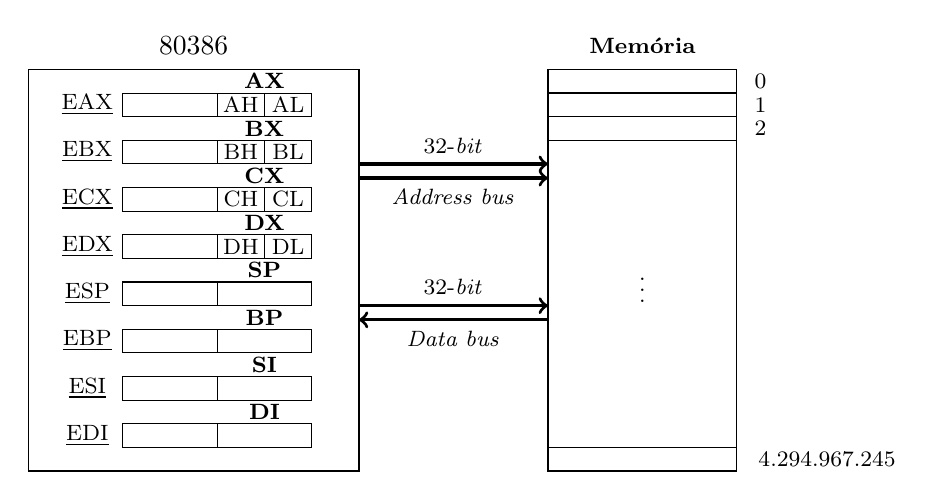
\begin{tikzpicture}[scale=0.6]
            \coordinate (A1) at (-3, 8);
            \coordinate (B1) at (4, 8);
            \coordinate (C1) at (4, -0.5);
            \coordinate (D1) at (-3, -0.5);

            \draw (A1) -- (B1) -- (C1) -- (D1) -- (A1);
            \node at (0.5, 8.5) { $80386$ };

            \draw (1, 7) rectangle (2, 7.5);
            \draw (2, 7) rectangle (3, 7.5);
            \draw (-1, 7) rectangle (1, 7.5);
            \node at (1.5, 7.25) { \footnotesize AH };
            \node at (2.5, 7.25) { \footnotesize AL };
            \node at (2, 7.75) { \footnotesize \bf AX };
            \node at (-1.75, 7.25) { \footnotesize \underline{EAX} };

            \draw (1, 6) rectangle (2, 6.5);
            \draw (2, 6) rectangle (3, 6.5);
            \draw (-1, 6) rectangle (1, 6.5);
            \node at (1.5, 6.25) { \footnotesize BH };
            \node at (2.5, 6.25) { \footnotesize BL };
            \node at (2, 6.75) { \footnotesize \bf BX };
            \node at (-1.75, 6.25) { \footnotesize \underline{EBX} };

            \draw (1, 5) rectangle (2, 5.5);
            \draw (2, 5) rectangle (3, 5.5);
            \draw (-1, 5) rectangle (1, 5.5);
            \node at (1.5, 5.25) { \footnotesize CH };
            \node at (2.5, 5.25) { \footnotesize CL };
            \node at (2, 5.75) { \footnotesize \bf CX };
            \node at (-1.75, 5.25) { \footnotesize \underline{ECX} };

            \draw (1, 4) rectangle (2, 4.5);
            \draw (2, 4) rectangle (3, 4.5);
            \draw (-1, 4) rectangle (1, 4.5);
            \node at (1.5, 4.25) { \footnotesize DH };
            \node at (2.5, 4.25) { \footnotesize DL };
            \node at (2, 4.75) { \footnotesize \bf DX };
            \node at (-1.75, 4.25) { \footnotesize \underline{EDX} };

            \draw (1, 3) rectangle (3, 3.5);
            \draw (-1, 3) rectangle (1, 3.5);
            \node at (-1.75, 3.25) { \footnotesize \underline{ESP} };
            \node at (2, 3.75) { \footnotesize \bf SP };

            \draw (1, 2) rectangle (3, 2.5);
            \draw (-1, 2) rectangle (1, 2.5);
            \node at (-1.75, 2.25) { \footnotesize \underline{EBP} };
            \node at (2, 2.75) { \footnotesize \bf BP };

            \draw (1, 1) rectangle (3, 1.5);
            \draw (-1, 1) rectangle (1, 1.5);
            \node at (-1.75, 1.25) { \footnotesize \underline{ESI} };
            \node at (2, 1.75) { \footnotesize \bf SI };

            \draw (1, 0) rectangle (3, 0.5);
            \draw (-1, 0) rectangle (1, 0.5);
            \node at (-1.75, 0.25) { \footnotesize \underline{EDI} };
            \node at (2, 0.75) { \footnotesize \bf DI };

            \coordinate (A2) at (8, 8);
            \coordinate (B2) at (12, 8);
            \coordinate (C2) at (12, -0.5);
            \coordinate (D2) at (8, -0.5);

            \coordinate (A3) at (8, 8);
            \coordinate (B3) at (12, 8);
            \coordinate (C3) at (12, 7.5);
            \coordinate (D3) at (8, 7.5);

            \coordinate (A4) at (8, 7.5);
            \coordinate (B4) at (12, 7.5);
            \coordinate (C4) at (12, 7);
            \coordinate (D4) at (8, 7);

            \coordinate (A5) at (8, 7);
            \coordinate (B5) at (12, 7);
            \coordinate (C5) at (12, 6.5);
            \coordinate (D5) at (8, 6.5);

            \coordinate (A6) at (8, 0);
            \coordinate (B6) at (12, 0);
            \coordinate (C6) at (12, -0.5);
            \coordinate (D6) at (8, -0.5);

            \draw (A2) -- (B2) -- (C2) -- (D2) -- (A2);
            \draw (A3) -- (B3) -- (C3) -- (D3) -- (A3);
            \draw (A4) -- (B4) -- (C4) -- (D4) -- (A4);
            \draw (A5) -- (B5) -- (C5) -- (D5) -- (A5);
            \draw (A6) -- (B6) -- (C6) -- (D6) -- (A6);

            \node at (10, 8.5) { \footnotesize \bf Memória };
            \node at (12.5, 7.75) { \footnotesize $0$ };
            \node at (12.5, 7.25) { \footnotesize $1$ };
            \node at (12.5, 6.75) { \footnotesize $2$ };
            \node[anchor=west] at (12.25, -0.25) { \footnotesize $4.294.967.245$ };
            \node at (10, 3.5) { \footnotesize $\vdots$ };
        
            \draw[->,very thick] (4, 6) -- node[anchor=south] { \footnotesize 32-\textit{bit} } (8, 6);
            \draw[->,very thick] (4, 5.7) -- node[anchor=north] { \footnotesize \textit{Address bus} } (8, 5.7); 
            \draw[->,very thick] (4, 3) -- node[anchor=south] { \footnotesize 32-\textit{bit} } (8, 3);
            \draw[<-,very thick] (4, 2.7) -- node[anchor=north] { \footnotesize \textit{Data bus} } (8, 2.7);
        \end{tikzpicture}
        \caption{Visualização parcial de um computador com processador 80386.\footnote{Fonte: \textbf{NEVELN}, Bob. \textit{Linux Assembly Language Programming}, Open Source Technology Series, Prentice-Hall, 2000 (com adaptações).}}
    \end{figure}

\end{frame}

